% Chapter 1
\chapter{ویژگی‌های نسخه جدید \lr{Openflow}}
همانگونه که در فصل قبل گفته شد، پروتکل \lr{Openflow} همواره در حال عرضه نسخه‌های جدید می‌باشد تا بتواند پاسخگوی نیاز‌ها به روز و پویای شبکه و همچنین رفع مشکلات نسخه‌های پیشین باشد. در شکل \ref{fig7} تغییرات عمده و مهم این پروتکل در بازه زمانی عرضه آن با نسخه \lr{OF1.0} تا هم اکنون (سال ۲۰۲۱ میلادی) که نسخه \lr{OF1.5.1} به صورت استاندارد قابل دسترس است را مشاهده می‌کنیم.

\begin{figure}[H]
	\centering
	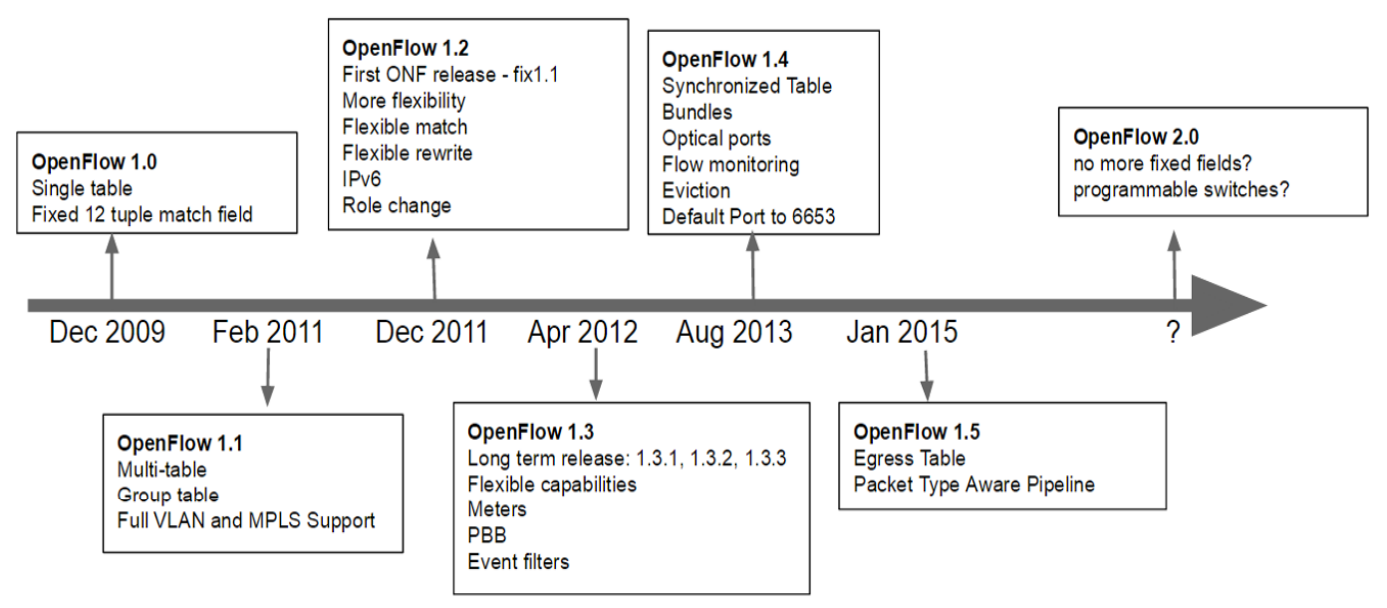
\includegraphics[scale=0.4]{imgs/of_timeline.png}
	\caption{روند پیشرفت پروتکل در نسخه‌های مختلف}
	\label{fig7}
\end{figure}

\pagebreak

\section{ویژگی‌های نسخه \lr{OF1.5}}
ویژگی‌های این نسخه را می‌توان در سه دسته، طبقه‌بندی کرد: اضافه شده‌ها، بهبود یافته‌ها و تغییرات. اضافه شده‌ها، ویژگی‌های کاملا جدیدی هستند که به پروتکل اضافه شده‌اند؛ بهبود یافته‌ها به منظور کامل کردن بخش‌های موجود در پروتکل اضافه شده اند و تغییرات نیز بخش‌هایی از پروتکل هستند که به صورت کامل دستخوش تغییر شده‌اند.
برخی از مهم‌ترین ویژگی‌های این نسخه عبارت‌اند از (تعدادی از ويژگی‌ها به دلیل جزئی بودن ذکر نشده است):

\begin{enumerate}[label=\Alph*]
	\item 
اضافه شده‌ها
	\begin{itemize}[noitemsep,topsep=0pt,parsep=0pt,partopsep=0pt]
		\item جداول جریان خروجی
		\item مهم بودن نوع بسته در خط لوله
		\item آماره‌های قابل انعطاف مرتبط با مدخل جریان \lr{(OXS)}
		\item ارسال خودکار آماره‌های مدخل جریان
		\item عملیات \lr{Copy-Field}
		\item تطابق \lr{TCP flags}
		\item وضعیت ارتباط کنترل کننده
	\end{itemize}
	\item
بهبود یافته‌ها
	\begin{itemize}[noitemsep,topsep=0pt,parsep=0pt,partopsep=0pt]
		\item دستورات تکاملی گروه برای تغییرات انتخابی در سطل‌ها
		\item اجازه استفاده از \lr{wildcard} در عملیات \lr{set-field}
		\item دسته‌های زمان‌بندی شده
	\end{itemize}
	\item
تغییرات
	\begin{itemize}[noitemsep,topsep=0pt,parsep=0pt,partopsep=0pt]
		\item تغییر \lr{Meter instruction} به \lr{Meter action}
	\end{itemize}
\end{enumerate}

در ادامه گزارش به شرح هر یک از تغییرات و کاربرد‌های آن‌ها می‌پردازیم.
\pagebreak

\subsection{جداول جریان خروجی}
در نسخه‌های قبلی تمام پردازش روی بسته‌ها در حیطه‌ی درگاه ورودی انجام می‌شد. اما در نسخه \lr{OF1.5} با معرفی جداول جریان خروجی\LTRfootnote{Egress Flow Tables}، قابلیت پردازش بسته‌ها در حیطه‌ی درگاه خروجی نیز فراهم می‌گردد. زمانی که بسته برای خروجی به درگاه مربوط ارجاع داده می‌شود، پردازش این بخش در اولین جدول جریان خروجی آغاز می‌شود که طی آن عملیات‌های مورد نظر روی بسته انجام شده یا به جداول دیگر خروجی ارجاع داده می‌شود. از ویژگی‌های این مرحله از پردازش می‌توان به موارد زیر اشاره کرد:
\begin{itemize}
	\item
تمام پردازش‌های مرتبط با پورت‌های منطقی، جداول جریان ورودی و جدول گروه قبل از این بخش انجام می‌شوند.
	\item
تعریف رفتار جدول جریان خروجی و مدخل‌های جریان آن بسیار شبیه به ورودی است.
	\item
قابلیت تغییر درگاه خروجی در این جداول وجود ندارد.
	\item
تمام فراداده‌های مربوط به خط لوله از پردازش  ورودی به پردازش خروجی منتقل می‌شوند.
	\item
مجموعه عملیات پردازش خروجی در ابتدا با عمل خروجی\LTRfootnote{Output action} پر شده است که در برابر مجموعه عملیات ورودی که تهی می‌باشد متفاوت است.
\end{itemize}
استفاده از پردازش قبل از خروجی از این جهت حائز اهمیت می‌باشد که در این مرحله از پردازش، درگاه خروجی و وضعیت نهایی بسته طی مراحل قبلی مشخص شده است و می‌توان عملیات‌های این بخش را با توجه به شرایط جدید انجام داد که این خود آزادی عمل بیشتری در تطابق و ایجاد تغییر در بسته‌ها را به ارمغان می‌آورد.

\subsection{مهم بودن نوع بسته در خط لوله}
در نسخه‌های قبلی، تمام بسته‌ها می‌بایست از نوع \lr{Ethernet} می‌بودند اما با معرفی نسخه \lr{OF1.5} قابلیت پردازش روی انواع مختلف بسته‌ها مانند بسته‌های \lr{IP} یا بسته‌های \lr{PPP} نیز فراهم گردید. فیلدی در خط لوله به منظور تطابق نوع بسته اضافه شده است که به عنوان پیش‌نیاز برای انجام تطابق فیلد‌های سرآیند می‌باشد. اضافه شدن این قابلیت، انعطاف تطابق را بالا برده و امکان تطبیق انواع وسیعی از بسته‌ها را در اختیار قرار می‌دهد که برای مثال توسط آن می‌توان برای انواع مختلف بسته‌ها کیفیت سرویس تنظیم کرد یا سیاست‌های امنیتی گسترده وضع نمود.

\pagebreak

\subsection{آماره‌های قابل انعطاف مرتبط با مدخل جریان \lr{(OXS)}}
در نسخه‌های قبلی، یک ساختار ثابت برای ذخیره آماره‌های مدخل جریان\LTRfootnote{Flow Entry Statistics} در نظر گرفته شده بود که در نسخه جدید با ساختار‌های انعطاف پذیر جایگزین شده است. با این تغییر، آماره‌های ذکر شده قابلیت جمع‌آوری و ذخیره داده‌های آماری دلخواه را خواهد داشت که امکان پایش و گزارش دقیق‌تر تغییرات و وضعیت شبکه را به پروتکل می‌دهد.

\subsection{ارسال خودکار آماره‌های مدخل جریان}
در نسخه‌های قبلی، کنترل کننده همواره به منظور دریافت آمار مدخل‌های جریان از سوئیچ نمونه‌برداری\LTRfootnote{Poll} داده به عمل می‌آورد که باعث ایجاد سربار پردازشی در سوئیچ می‌گردید. در نسخه جدید، آماره‌های فوق الذکر، به صورت خودکار در صورت عبور از آستانه‌های تعریف شده به کنترل کننده گزارش داده می‌شوند.

\subsection{عملیات \lr{Copy-Field}}
عملیات \lr{Set-Field} موجود در پروتکل امکان تنظیم یک مقدار ثابت را در فیلد‌های سرآیند و خط لوله فراهم می‌کند. عملیات جدید \lr{Copy-Field} امکان رونوشت فیلد‌های سرآیند و خط لوله را از بسته‌ای به بسته دیگر فراهم می‌کند که این خود باعث کاهش تعداد عملیات انجام شده و کاهش سربار پردازشی می‌گردد.

\subsection{تطابق \lr{TCP flags}}
قابلیت تطابق با پرچم‌های موجود در سرآیند بسته‌های \LTRfootnote{TCP} در این نسخه اضافه شده است. این قابلیت، انعطاف انجام تطابق را برای پروتکل افزایش می‌دهد و از آن می‌توان به منظور پیاده‌سازی سیاست‌های مربوط به درخواست‌ها یا وضع سیاست‌های امنیتی جهت جلوگیری از انواع حمله استفاده کرد.

\subsection{وضعیت ارتباط کنترل کننده}
وضعیت ارتباط کنترل کننده، این امکان را به کنترل کننده می‌دهد تا درباره تمام ارتباطات سوئیچ با کنترل کننده‌های دیگر مطلع شود. این ویژگی به همراه قابلیت چند کنترل کننده بودن سوئیچ اجازه قسمت بندی شبکه کنترل کننده‌ها و پایش وضعیت کنترل کننده‌های دیگر را به ارمغان می‌آورد. هر کنترل کننده خود را به یک شناسه کوتاه تشخیص می‌دهد و کنترل کننده‌های دیگر را توسط آدرس \lr{URI} از یکدیگر متمایز می‌کند.
\pagebreak

\subsection{دستورات تکاملی گروه برای تغییرات انتخابی در سطل‌ها}
در نسخه‌های قبلی، به منظور ایجاد تغییر در سطل‌های موجود در گروه، تمام مجموعه سطل‌ها تحت تاثیر قرار می‌گرفت. دو دستور درج کردن\LTRfootnote{Insert} به منظور اضافه کردن سطل به گروه و حذف کردن\LTRfootnote{Remove} به منظور حذف سطل از گروه به مجموعه دستورات گروه اضافه گردید که باعث کاهش عملیات و سربار پردازش در انجام عملیات مرتبط با گروه می‌شود.

\subsection{اجازه استفاده از \lr{wildcard} در عملیات \lr{set-field}}
در نسخه‌های قبلی، به منظور تغییر فیلد با استفاده از عملیات \lr{set-field} تمام بخش‌های فیلد مورد نظر باید تنظیم می‌شد اما به اضافه شدن قابل \lr{wildcard} می‌توان بخش‌های بدون تغییر فیلد را پوشاند تا نیازی به تنظیم دوباره آن نباشد.

\subsection{دسته‌های زمان‌بندی شده}
در نسخه \lr{OF1.4}، ویژگی جدیدی به نام \lr{Bundles} معرفی شد که طبق آن گروهی از پیام‌های \lr{Openflow} طی یک عملیات اجراء می‌شوند. این قابلیت به کنترل کننده‌ها امکان ایجاد همزمان دستورات مرتبط را می‌دهد که باعث موجب هماهنگی و همزمانی بین سری سوئیچ‌ها می‌گردد. در این دسته از دستورات، در صورت بروز خطا در یک دستور، تمام دسته با شکست مواجه می‌شود که این عامل اصلی ایجاد هماهنگی بین سوئیچ‌ها است.\\
حال در نسخه\lr{OF1.5}، ویژگی دسته‌های زمان‌بندی شده\LTRfootnote{Scheduled Bundles} این امکان را فراهم می‌آورد که بتوان برای اجراء دستورات موجود در دسته، زمان مشخصی تنظیم کرد.

\subsection{تغییر \lr{Meter instruction} به \lr{Meter action}}
در نسخه‌های قبلی، عمل اندازه‌گیری توسط یک دستور اندازه‌گیری انجام می‌گرفت اما در نسخه جدید این امکان توسط عملیات اندازه‌گیری صورت می‌پذیرد که این تغییر، قابلیت اضافه کردن چندین اندازه‌گیر به مدخل جریان و قابلیت اضافه کردن اندازه‌گیر به گروه‌ها را به پروتکل می‌دهد. کاربرد این قابلیت در اعمال سیاست‌های مرتبط با اندازه‌گیری‌های چندگانه بر روی ترافیک ورودی سوئیچ می‌باشد که انعطاف بالاتری را به شبکه می‌افزاید.
\pagebreak

\section{وضعیت پشتیبانی از نسخه‌ها}
پروتکل \lr{Openflow} در مسیر پیشرفت، با مشکلات بزرگی مواجه می‌شود. یکی از مشکلات این است که شرکت‌های تولید کننده نرم‌افزار و سخت‌افزار به دلیل وسعت دامنه تغییرات برای پشتیبانی، نمی‌توانند با سرعت پیشرفت پروتکل هماهنگ شوند. و مشکل دوم نیز از آنجایی نشئت می‌گیرد که پروتکل \lr{Openflow} تلاش دارد تا اکوسیستمی برای شبکه فراهم آورد که از تولید کننده سخت‌افزار مجزا است و در آن تجهیزات از شرکت‌های تولید کننده مختلف می‌توانند تحت یک کنترل کننده عمل کنند اما پس از عرضه پروتکل مشاهده می‌شود که حتی نسخه یکسانی از پروتکل که توسط چند شرکت متفاوت پیاده سازی شده‌اند نیز دارای تفاوت‌هایی در عملکرد و پیکربندی می‌باشد.\\
در زمان نگارش این گزارش، نسخه \lr{OF1.3} به صورت گسترده در تجهیزات و کنترل کننده‌های عملیاتی در حال استفاده است. نسخه \lr{OF1.4} در حال افزایش پشتیبانی و تعداد استفاده تجهیزات از آن است که در آینده نزدیک شاهد جایگزینی کامل \lr{OF1.3} با این نسخه خواهیم بود. اما با تغییرات عمده صورت گرفته در نسخه \lr{OF1.5} به ویژه تغییرات در خط لوله و اضافه شدن مرحله پردازشی خروجی، انتظار می‌رود روند همه‌گیر شدن استفاده از این نسخه به کندی صورت پذیرد. در حال حاضر سوئیچ‌های نرم‌افزاری مانند \lr{OVS} و برخی از برند‌های سخت افزار از این پروتکل پشتیبانی می‌کنند اما هیچ یک از کنترل کننده‌های موجود قادر به شناسایی این نسخه نمی‌باشند.


